\documentclass[12pt]{article}

\usepackage[preprint]{neurips_2021}

\usepackage[utf8]{inputenc} % allow utf-8 input
\usepackage[T1]{fontenc}    % use 8-bit T1 fonts
\usepackage{hyperref}       % hyperlinks
\usepackage{url}            % simple URL typesetting
\usepackage{booktabs}       % professional-quality tables
\usepackage{amsfonts}       % blackboard math symbols
\usepackage{nicefrac}       % compact symbols for 1/2, etc.
\usepackage{microtype}      % microtypography
\usepackage{xcolor}

\usepackage{amsmath}

\usepackage{graphicx}

\graphicspath{ {./images/} {./images/ae/} {./images/bad/} {./images/curves/} {./images/latent/} {./images/raw/} }

\usepackage{amsthm}
\newtheorem{definition}{Definition}

\usepackage{float}

\newcommand{\contentdescription}[1]{}

\newcommand{\TODO}[2]{{#2}}

\title{Generating 3D Point Cloud Data with Generative Adversarial Networks and Autoencoders}

\author{
    Pavlo Melnyk$^*$ \\
    \texttt{pavlo.melnyk@liu.se} \\
    \And
    Julian Alfredo Mendez$^\star $ \\
    \texttt{julian.mendez@umu.se} \\
    \And
    Emanuel S\'{a}nchez Aimar$^*$ \\
    \texttt{emanuel.sanchez.aimar@liu.se} \\
    \\
    {\small $^*$Computer Vision Laboratory, Department of Electrical Engineering, Linköping University} \\
    {\small $^\star$ Department of Computing Science, Umeå University}
}

\begin{document}

    \maketitle

    \begin{abstract}
        \contentdescription{
            Abstract (5-10\%):
            Give an overview of what you have done in the project with the key results and findings of your work.
            Should be no more than 300 words.
        }

        Recognition and representation of 3D geometric data is a challenging and fruitful topic that has fast developed in recent years. An intuitive way to represent such type of data is as a set of 3D locations in a Euclidean coordinate frame, i.e., as a \textit{point cloud}. However, as for other types of data, generating 3D point clouds possess a unique set of challenges, which inspired us consider this task.
        In this report,  we analyze and implement the raw and latent generative adversarial network (r- and l-GAN, respectively) methods proposed in the original work~\cite{pmlr-v80-achlioptas18a} to generate point clouds of 3D shapes of different categories using the ShapeNet data. The main feature of the latter is the use of a deep autoencoder (AE) network that is trained by minimizing the Chamfer pseudo-distance and has ``state-of-the-art reconstruction quality and generalization ability''.
        Importantly, apart from (subjective) qualitative assessment of the generated geometric data, we perform quantitative evaluation of the generative models by using the introduced measures of sample fidelity (i.e., \textit{minimum matching distance}) and diversity (i.e., \textit{coverage}) based on matchings between sets of point clouds.
        The original work implementation\footnote{\url{https://github.com/optas/latent_3d_points}} is in TensorFlow\footnote{\url{https://www.tensorflow.org/}}, whereas we use PyTorch\footnote{\url{https://pytorch.org}} to build the models and conduct experiments.
    \end{abstract}


    \section{Introduction}

    \contentdescription{
        Introduction (5-15\%):
        Describe the problem, the approach of the paper, the experiments, and the results.
        At the high-level talk about what you worked on in your project and why it is important.
        Then give an overview of your results.
    }

    The applications of representing three-dimensional (3D) images are numerous, like its use in augmented and virtual reality.
    In turn, these can be applied on a variety of domains, ranging from medicine to gaming.

    One of the critical problems of 3D sampling is the different rotations an image can have.

    We applied three approaches: raw GAN, autoencoder, and l-GAN, which are defined in the subsequent sections.

    This report presents analysis and the results of a reimplementation of~\cite{pmlr-v80-achlioptas18a} using PyTorch.


    \section{Related work}
    \contentdescription{
        Related Work (5-15\%):
        Discuss the published work related to your project paper, the types of experiments you do and the additional method that you have added to this work or you have compared this paper with (if any).
    }


    Some of the deep architectures for 3D point clouds in the literature focus in classification and segmentation.
    That is the case with PointNet~\cite{arxiv:1612.00593},
    which is ``a unified architecture for applications ranging from object classification, part segmentation, to scene semantic parsing''.
    It is a novel type of neural networks that takes point clouds as input and respects the permutation invariance of points for that input.

    Their architecture is based on autoencoders (AEs)\cite{doi:10.5555/65669.104451}\cite{arxiv:1312.6114},
    and generative adversarial networks (GANs)\cite{NIPS2014_5ca3e9b1}\cite{arxiv:1511.06434}\cite{arxiv:1612.02136}.
    These techniques were used to generate samples from complex underlying distributions.


    \section{Methods}
    \contentdescription{
        Methods (15-25\%):
        Describe the original paper's method to the extent that you would need to make your report and findings understandable.
        Otherwise, here you can describe other methods that you compare with or other methods that you apply on top of what you reimplemented.
        Here, you also try to justify any methodical modification or incremental changes that you have added to the original paper.
        It may be helpful to include figures, diagrams, or tables to describe your method or compare it with other methods.
    }

    To facilitate the reader's understanding of the original work, as well as the content of Sections~\ref{sec:data_experiments_findings}~and~\ref{sec:conclusions} of our report, we describe the main concepts in the form of definitions below.

    \begin{definition}
        \normalfont
        A \emph{point cloud} is a set of points $(x, y, z)$ in a Euclidean coordinate frame.
    \end{definition}

    In this paper, a point cloud usually represents a surface.

    \begin{definition}
        \normalfont
        A \emph{metric} or \emph{distance function} is a function defined
        $d: X \times X \to \mathbb{R}_{\geq 0}$
        with the following properties:

        \begin{enumerate}
            \item $d(x,y) = 0 \Leftrightarrow x = y$
            \item $d(x,y) = d(y,x)$
            \item $d(x,y) \leq d(x,z) + d(z,y)$
        \end{enumerate}

        A \emph{pseudo-distance} has similar properties, but it allows different points to have distance 0, and the first requirement is replaced by:
        \[d(x,x) = 0\]
    \end{definition}

    \begin{definition}
        \normalfont
        The \emph{Chamfer (pseudo)-distance (CD)} between point clouds $S_1$ and $S_2$ is defined as follows:

        \begin{equation}
            d_{CD}(S_{1}, S_{2}) =
            \sum_{x \in S_{1}} \min _{y \in S_{2}} || x - y||_{2}^{2} + \sum_{y \in S_{2}} \min_{x \in S_{1}} ||x - y||_{2}^{2}
            \label{equation:chamfer_distance}
        \end{equation}

    \end{definition}

    % The EMD and the CD are used to measure the sampling error of the results.

    In this work, the application of CD is two-fold. First, CD defines a reconstruction loss to train autoencoders presented in definition 4. Second, following the original paper, we implement high level metrics in definition 7 and 8, namely fidelity and coverage, in terms of CD.

    \begin{definition}
        \normalfont
        The \emph{autoencoder} architecture is a design to reconstruct its input, and is composed by an \emph{encoder} (E) and a \emph{decoder} (D). The pipeline is represented in Figure~\ref{figure:diagram_of_autoencoder}.
        % \[x \to E \to z \to D \to \hat{x}\]

        \begin{figure}[H]
            \centering
            \begin{tabular}{cc}
                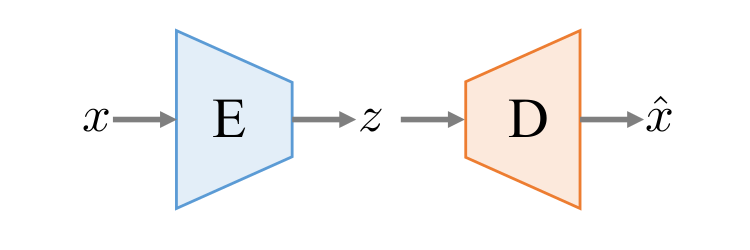
\includegraphics[width = 50mm]{autoencoder}
            \end{tabular}
            \caption{Diagram of an autoencoder as described in~\cite{pmlr-v80-achlioptas18a}.}
            \label{figure:diagram_of_autoencoder}
        \end{figure}

        The encoder takes an input $x$ and produces a compressed version $z$, which is called the \emph{latent representation} of $x$. The decoder tries to reconstruct $x$ by using $z$ as input, and returns $\hat{x}$ as output.
    \end{definition}

    The basic architecture used in this paper is the generative adversarial networks (GANs).

    \begin{definition}
        \normalfont
        A \emph{generative adversarial network} (GAN) \cite{NIPS2014_5ca3e9b1} is an interplay between a \emph{generator} (G) and a \emph{discriminator} (D).
        In that interaction, the generator tries to synthesize samples that mimic real data by giving a randomly created sample through the generator function, while the discriminator needs to distinguish the synthesized examples from the real ones. This adversarial process is illustrated in Figure~\ref{figure:diagram_of_gan}. During training, we alternate the optimization of the losses presented in Eq. \ref{equation:disc_loss} and Eq. \ref{equation:gen_loss} for the discriminator and generator, respectively.

        \begin{figure}[H]
            \centering
            \begin{tabular}{cc}
                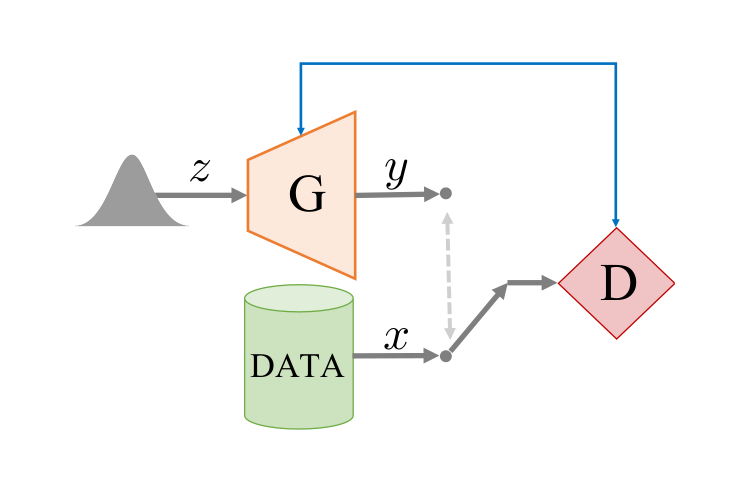
\includegraphics[width = 50mm]{gan}
            \end{tabular}
            \caption{Diagram of a GAN as described in~\cite{pmlr-v80-achlioptas18a}.}
            \label{figure:diagram_of_gan}
        \end{figure}

        \begin{equation}
            \mathcal{L}_{dis} = \mathop{\mathbb{E}}_{x \sim p_x(x)}[log D(x)] + \mathop{\mathbb{E}}_{z \sim p_z(z)}[log (1 - D(G(z))]
            \label{equation:dis_loss}
        \end{equation}

        \begin{equation}
            \mathcal{L}_{gen} = \mathop{\mathbb{E}}_{z \sim p_z(z)}[log D(G(z))]
            \label{equation:gen_loss}
        \end{equation}

    \end{definition}

    \begin{definition}
        \normalfont
        \textit{Permutation invariance} of a point cloud implies that any reordering of the points yields a point cloud that represents the same shape. This complicates comparisons between two point sets which is needed to define a reconstruction loss, as noted in~\cite{pmlr-v80-achlioptas18a} and requires a permutation invariant learning of encoded features.

        We say that a model (e.g., a neural network classifier) is \emph{permutation invariant} when it does not assume any spatial relationships between the features in the input. E.g., if one permutes the points in the input point set and the performance of the model remains the same, then the model is permutation invariant.
        The generative models considered in this work are permutation invariant by construction since they contain 1-D convolutional layers with kernel size 1, allowing encoding the points \textit{independently}, and a symmetric (permutation invariant) max-pooling operation over the feature dimension.
        % ...
    \end{definition}

    \begin{definition}
        \normalfont
        Given two sets of point clouds $A$ and $B$, and given a distance, we say that \emph{coverage} is a measure for the fraction of the point clouds in $B$ that were matched to point clouds in $A$, such that each point cloud in $A$ is related to its the closest neighbor in $B$ using the given distance.
    \end{definition}

    \begin{definition}
        \normalfont
        We define the \emph{fidelity} of $A$ with respect to $B$ as the \emph{minimum matching distance} (MMD) of matching each point in $B$ to a point in $A$.
        The \emph{MMD} is computed as an average of the individual point-wise distances, using either the CD or EMD.
        They are called the \emph{MMD-CD} and \emph{MMD-EMD} respectively.
    \end{definition}

    Fidelity and coverage are meant to measure the global error of the computation.

    Let us see an intuitive example behind fidelity and the MMD.
    If we sample chairs, we can look at the closest matching chair from the generated ones for a given metric.


    \section{Data, experiments and findings}
    \label{sec:data_experiments_findings}
    \contentdescription{
        Data, experiments and findings (30-40\%):
        Describe the data you are working with for your project.
        What type of data is it?
        Where did it come from?
        How much data are you working with?
        Did you have to do any preprocessing, filtering, or other special treatment to use this data in your project?
        Describe and present the experiments that you performed and what is the reason for those experiments.
        Where applicable define evaluation metrics that you used. Discuss the results that you got.
    }

    Following the original work \cite{pmlr-v80-achlioptas18a}, we use the ShapeNet dataset~\cite{arxiv:1512.03012} consisting of 16 classes of shapes
    %(\verb|"Airplane", "Bag", "Cap", "Car", "Chair", "Earphone", "Guitar", "Knife", "Lamp", "Laptop", "Motorbike", "Mug", "Pistol", "Rocket", "Skateboard", "Table"|)
    that are axis aligned and centered into the unit sphere, and provided as point clouds in the PyTorch Geometric\footnote{\url{https://pytorch-geometric.readthedocs.io/en/latest/}} package.
    For example, Figure~\ref{figure:cars_from_shapenet} shows two cars taken from the ShapeNet dataset.

    \begin{figure}
        \centering
        \begin{tabular}{cc}
            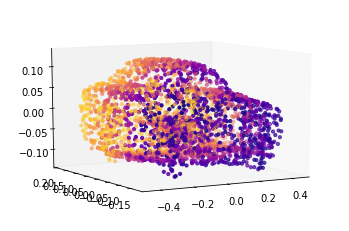
\includegraphics[width = 50mm]{car-shapenet-1} &
            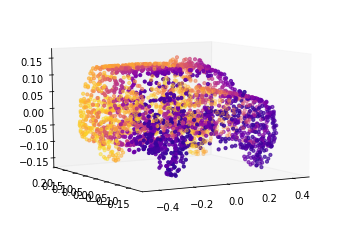
\includegraphics[width = 50mm]{car-shapenet-2} \\
        \end{tabular}
        \caption{Two car samples from the ShapeNet dataset.}
        \label{figure:cars_from_shapenet}
    \end{figure}

    We use shapes of one class and uniformly sample 2048 points from each point cloud to train models. We use the default ``trainval'' set (i.e., training + validation data) for training, and compute the metrics on the test set (i.e., \verb|split="test"|).

    We conduct two types of experiments: with raw GANs (\textit{r-GANs}) and latent GANs (\textit{l-GANs}). In the latter, we use deep AEs to learn the encoding of the point clouds. The architectures of all models are replicated from the original work (see Appendix in \cite{pmlr-v80-achlioptas18a} and the model summary outputs in the notebooks that we provide in the supplementary material). The important feature of the r-GAN generator and the encoder part of the AE are 1-D convolutional layers that allow applying the learned parameters feature-wise \textit{independently}.

    \subsection{r-GAN experiments} As the name suggests, this type of GAN operates on the raw data, i.e., a $2048 \times 3$ matrix representing a 3D shape. We use the hyperparameters to train the r-GAN that are suggested in the original work, but stop the optimization after 200 epochs (instead of the suggested 2000) for the sake of computational efficiency. The generator takes as input a random vector of length $128$ sampled from $\mathcal{N}(0,0.04)$.
    The generated samples of the shapes of categories \verb|Lamp|, \verb|Table|, and \verb|Chair| are presented in Figure~. Some graphs of the generator and discriminator losses (defined by \eqref{equation:gen_loss} and \eqref{equation:dis_loss}, respectively) are presented in Figure~.
    The quantitative results for the samples, i.e., the fidelity and coverage scores for the corresponding generated and test point cloud sets are shown in Table~\ref{table:results}.

    \subsection{l-GAN experiments} Instead of utilizing the raw data, the l-GAN takes as input the encoding of the raw data. The encoding of a raw point-cloud is obtained by passing the data through the encoder part of a pretrained AE trained for each shape separately by minimizing the CD loss function~\eqref{equation:chamfer_distance}.

    We can describe our experiments with l-GANs using the following 3 stages:
    \textbf{Stage 1} For a given shape category, train an autoencoder by minimizing the CD loss~\eqref{equation:chamfer_distance} between the input and reconstructed point clouds. The output of the encoder, the bottleneck $z$, represents the compressed representation, i.e., \textit{encoding}.
    % For comparison, in the raw GAN approach, a point cloud is used instead of a compressed representation.
    \textbf{Stage 2} We sample a Gaussian distribution $\mathcal{N}(0,\sigma)$.


    \textbf{Stage 3}
    This is used to sample and create using GANs
    $C' = \sigma(z)$
    $P = D(C')$

    We used examples of a chair, a table, and an airplane.
    Figure~\ref{figure:car_sampled_with_lGAN} show an example of a car sample generated with l-GAN.

    \begin{figure}
        \centering
        \begin{tabular}{cc}
            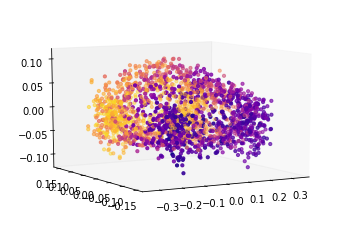
\includegraphics[width = 50mm]{car-lgan}
        \end{tabular}
        \caption{Car sample generated with l-GAN.}
        \label{figure:car_sampled_with_lGAN}
    \end{figure}


    \begin{figure}
        \centering
        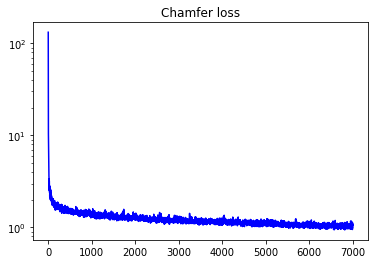
\includegraphics[width = 50mm]{chamfer-loss}
        \caption{Chamfer loss.}
        \label{figure:chamfer_loss}
    \end{figure}


    \begin{table}[H]
        \caption{Results.}
        \centering
        \begin{tabular}{lll}
            \toprule
            Model          & Fidelity $\downarrow$ & Coverage $\uparrow$ \\
            \midrule
            r-GAN Chair    & 0.0022                & 14.35               \\
            l-GAN Chair    & 0.0017                & 38.21               \\
            \midrule
            r-GAN Lamp     & 0.0196                & 17.48               \\
            l-GAN Lamp     & 0.0058                & 18.18               \\
            \midrule
            r-GAN Table    & 0.023                 & 22.05               \\
            l-GAN Table    & 0.002                 & 34.91               \\
            \midrule
            r-GAN Airplane & 0.001                 & 12.02               \\
            l-GAN Airplane & 0.0007                & 27.27               \\
            \bottomrule
        \end{tabular}
        \label{table:results}
    \end{table}

    \subsection{Results}

    As we can see from Figure~, the quality of the resulting r-GAN generated samples of \verb|Table| and \verb|Chair| is reasonably good, considering the 10-fold shorter optimization we performed compared to the baseline. However, the r-GAN generating samples of \verb|Lamp| does not produce as good point clouds. This is well reflected by the generator and discriminator loss graph displayed in Figure~. A possible reason for this phenomenon is the amount of training data: we observe a strong correlation between the number of training samples and the quality of shapes generated.




    \begin{figure}
        \centering
        \begin{tabular}{lllllll}
            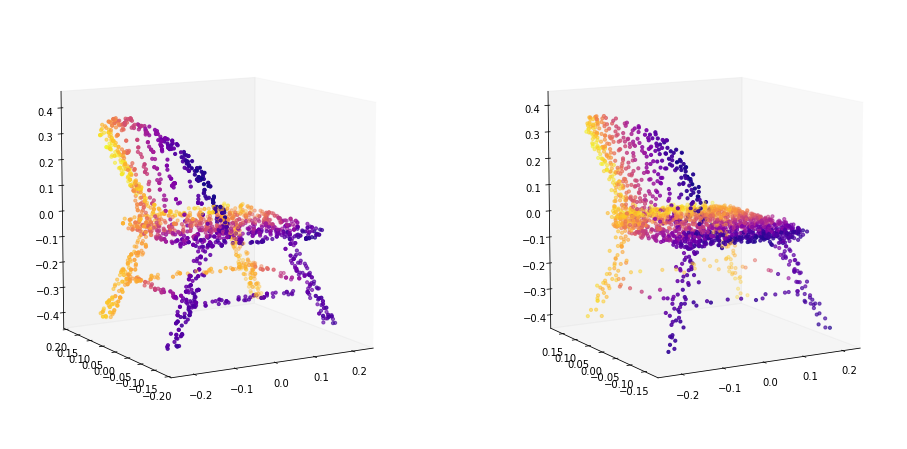
\includegraphics[width = 60mm]{chair_ae_1} &
            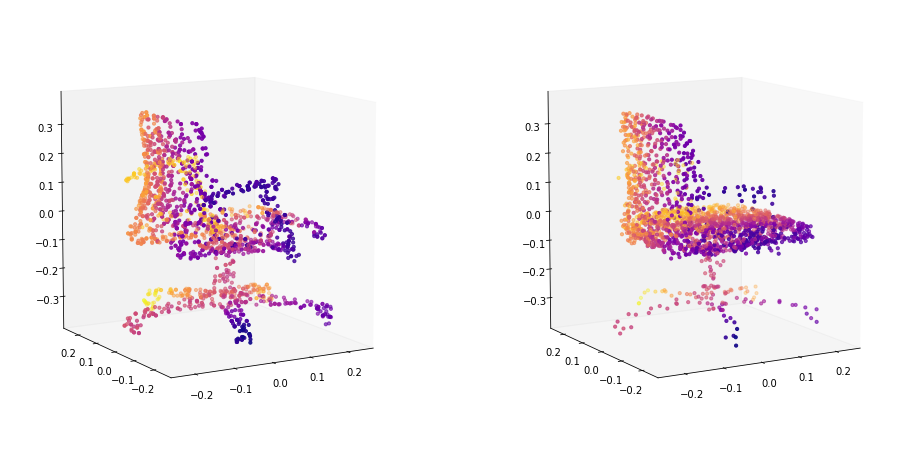
\includegraphics[width = 60mm]{chair_ae_2} \\
            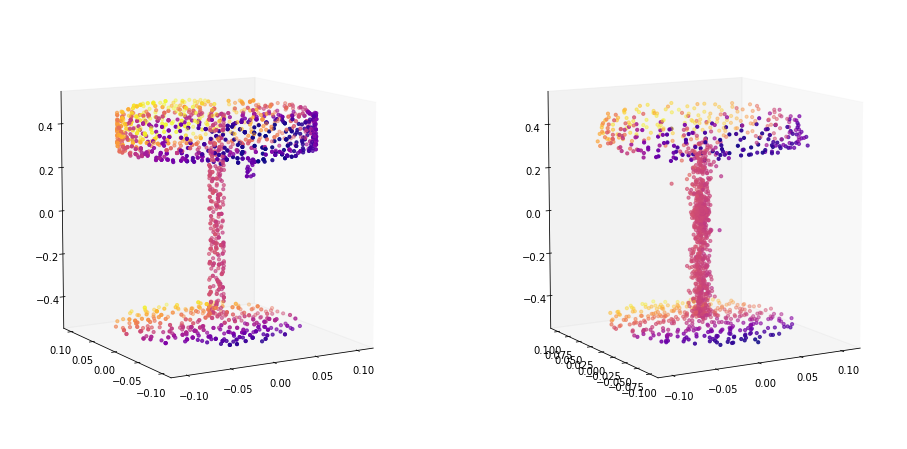
\includegraphics[width = 60mm]{lamp_ae_1} &
            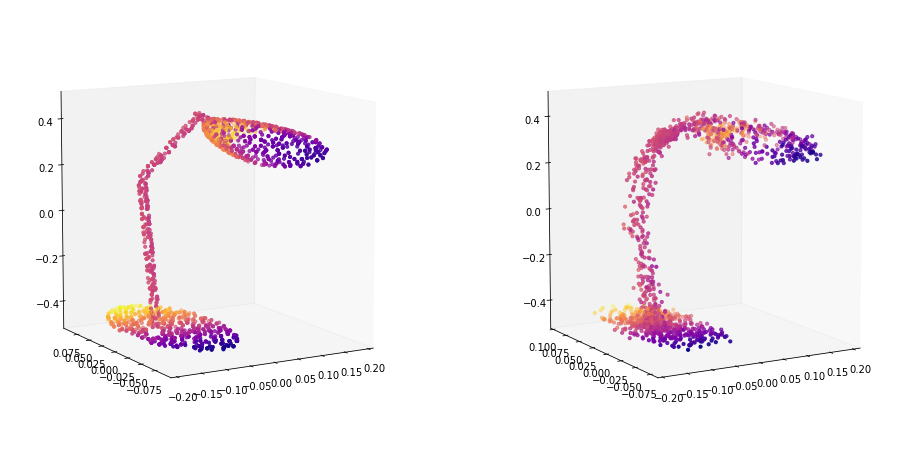
\includegraphics[width = 60mm]{lamp_ae_2} \\
            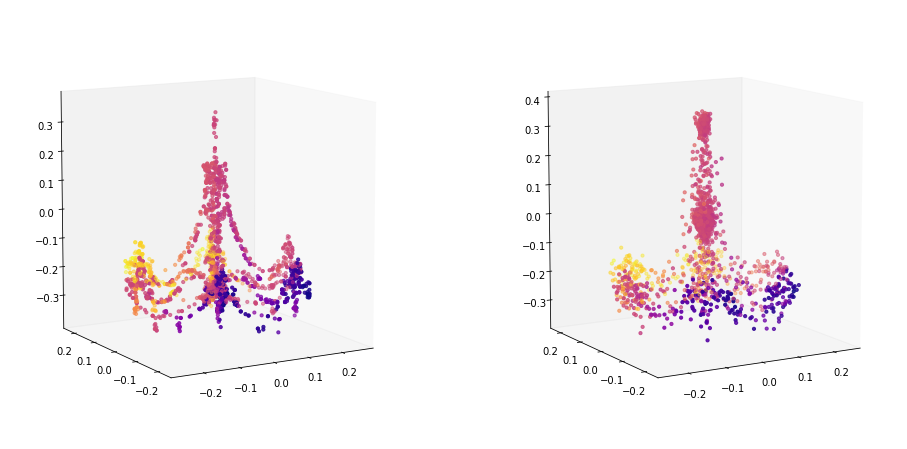
\includegraphics[width = 60mm]{lamp_ae_3} \\
            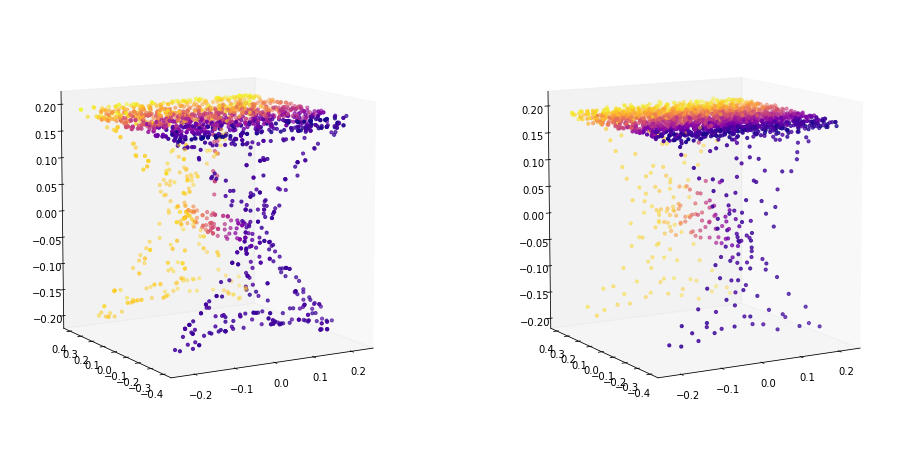
\includegraphics[width = 60mm]{table_ae_1} &
            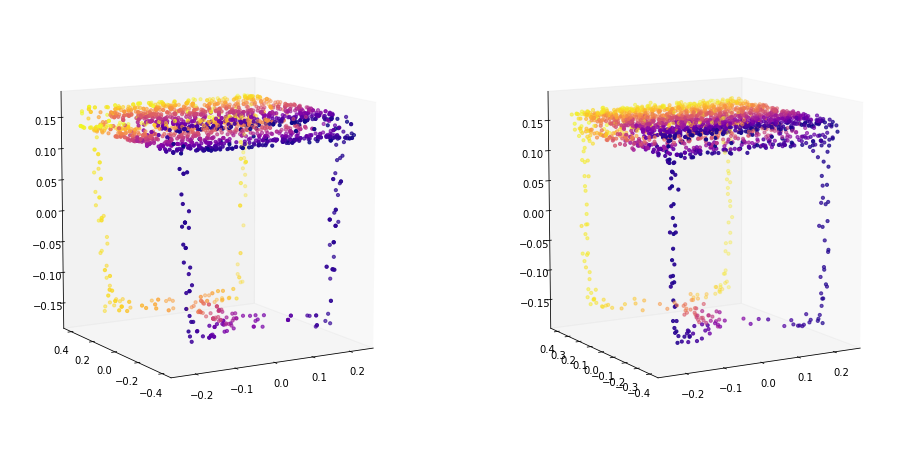
\includegraphics[width = 60mm]{table_ae_2} \\
        \end{tabular}
        \caption{Samples generated with autoencoders.}
        \label{figure:samples_generated_with_autoencoders}
    \end{figure}


    \begin{figure}
        \centering
        \begin{tabular}{lllllll}
            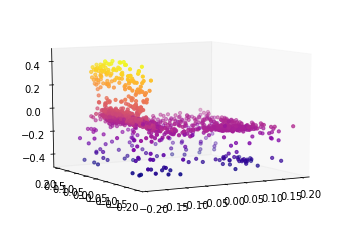
\includegraphics[width = 30mm]{chair_raw_gen_1} &
            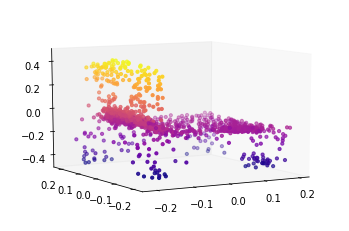
\includegraphics[width = 30mm]{chair_raw_gen_2} &
            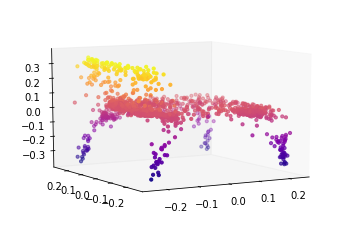
\includegraphics[width = 30mm]{chair_raw_gen_3} \\
        \end{tabular}
        \caption{Samples generated with raw GAN.}
        \label{figure:samples_generated_with_raw_gan}
    \end{figure}


    \begin{figure}
        \centering
        \begin{tabular}{lllllll}
            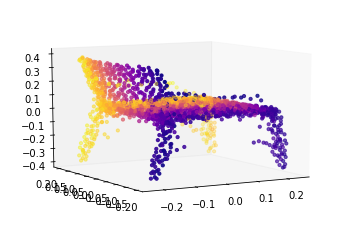
\includegraphics[width = 30mm]{chair_latent_gen_1} &
            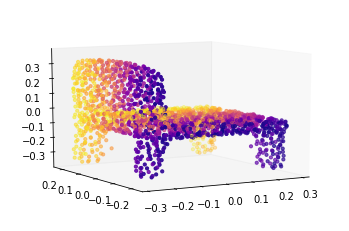
\includegraphics[width = 30mm]{chair_latent_gen_2} &
            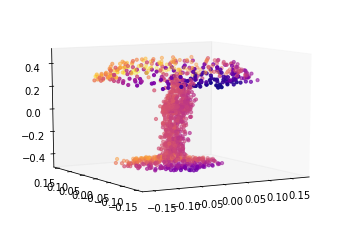
\includegraphics[width = 30mm]{lamp_latent_gen_1} &
            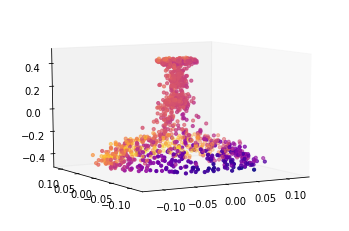
\includegraphics[width = 30mm]{lamp_latent_gen_2} \\
            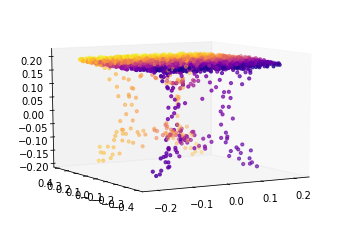
\includegraphics[width = 30mm]{table_latent_gen_1} &
            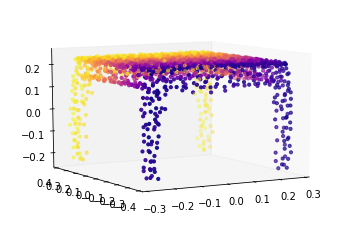
\includegraphics[width = 30mm]{table_latent_gen_2} &
            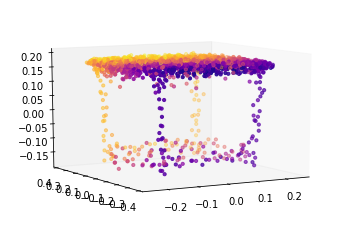
\includegraphics[width = 30mm]{table_latent_gen_4} \\
        \end{tabular}
        \caption{Samples generated with latent GAN.}
        \label{figure:samples_generated_with_latent_gan}
    \end{figure}


    \begin{figure}
        \centering
        \begin{tabular}{lllllll}
            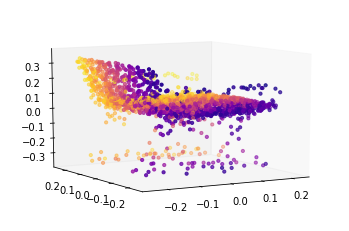
\includegraphics[width = 30mm]{chair_latent_gen_3_bad} &
            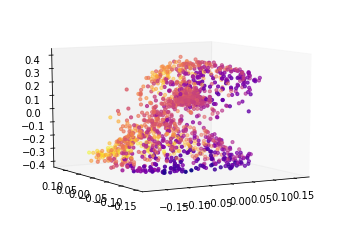
\includegraphics[width = 30mm]{lamp_latent_gen_3_bad} &
            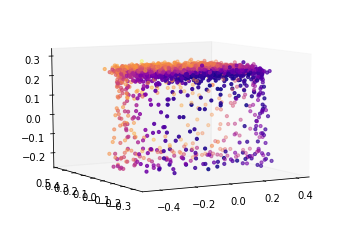
\includegraphics[width = 30mm]{table_latent_gen_3_bad} \\
        \end{tabular}
        \caption{Bad samples generated with latent GAN.}
        \label{figure:bad_samples_generated_with_latent_gan}
    \end{figure}


    \begin{figure}
        \centering
        \begin{tabular}{lllllll}
            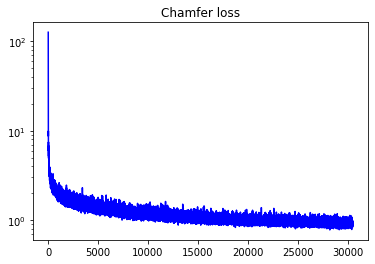
\includegraphics[width = 30mm]{chair_l_gan_curves} &
            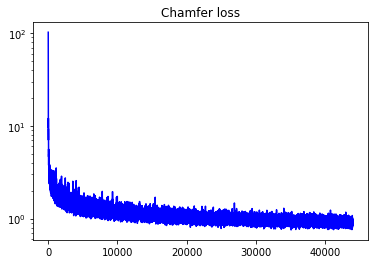
\includegraphics[width = 30mm]{table_l_gan_curves} &
            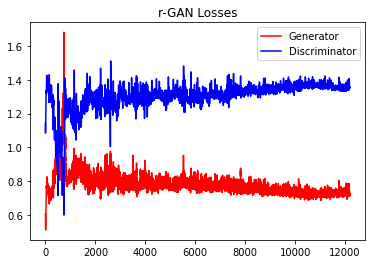
\includegraphics[width = 30mm]{chair_raw_gan_curves} &
            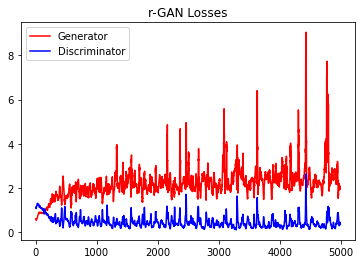
\includegraphics[width = 30mm]{lamp_raw_gan_curves} \\
        \end{tabular}
        \caption{Curves for latent GAN and raw GAN.}
        \label{figure:curves_for_latent_gan_and_raw_gan}
    \end{figure}


    \section{Challenges and conclusions}
    \label{sec:conclusions}
    \contentdescription{
        Challenges and Conclusions (5-15\%):
        Challenges you faced when reimplementing the paper and conducting the experiments.
        Were all details in the paper?
        Or did you have to look in the authors code or even contact them to find about some details?
        Was parts of the code quite hard to get them to work as intended?
        Did you have optimize and tune several hyperparameters?
        Which ones?
        Did the framework you used make the implementation difficult in some ways?

        Summarize your key results - what have you learned?
        What points do you think one should consider when using the approach of the paper you chose for your project?
        Suggest ideas for future extensions or new applications of your ideas.
    }

    We are able to successfully reproduce the results in~\cite{pmlr-v80-achlioptas18a}.

    Utilizing the latent space GANs (l-GANs), we can achieve better reconstructions, as discussed in the original work.
    By contrast, the raw GAN performance is considerably lower when not enough data is provided.

    For example, in some of our experiments we found that the lamp data were insufficient to train the raw GAN reasonably well.


    \section{Ethical consideration, societal impact, potential alignment with UN SDGs}
    \contentdescription{
        Ethical consideration, societal impact, potential alignment with UN SDGs (5-10\%):
        Think and research!
        Are there any ethical considerations for the original paper, its problem or method, its way of conducting experiments?
        How about your task, your datasets, and the experiments you did?
        What societal impact can you imagine about the original paper and its contributions and results?
        How about your project report?
        How do you think this paper can push the UN SDG targets?
    }

    The Sustainable Development Goals (SDGs), were adopted by the United Nations in 2015 as a universal call
    to end poverty and protect the planet\footnote{\url{https://sdgs.un.org/goals}}, intended to be achieved by the year 2030.
    % For the sake of completeness, we mention the goals:
    % \begin{enumerate}
    %    \item No Poverty,
    %    \item Zero Hunger,
    %    \item Good Health and Well-being,
    %    \item Quality Education,
    %    \item Gender Equality,
    %    \item Clean Water and Sanitation,
    %    \item Affordable and Clean Energy,
    %    \item Decent Work and Economic Growth,
    %    \item Industry, Innovation and Infrastructure,
    %    \item Reducing Inequality,
    %    \item Sustainable Cities and Communities,
    %    \item Responsible Consumption and Production,
    %    \item Climate Action,
    %    \item Life Below Water,
    %    \item Life On Land,
    %    \item Peace, Justice, and Strong Institutions,
    %    \item Partnerships for the Goals.
    %\end{enumerate}

    Use of GANs can impact indirectly in all of the goals.
    However, we have chosen three items, which we consider the most directly affected:
    \textbf{Decent Work and Economic Growth}, \textbf{Industry, Innovation and Infrastructure}, and
    \textbf{Sustainable Cities and Communities}.

    We base our position on the fact ethical uses of machine learning can have a positive impact in societal development.
    Technology can leave humans in overseeing positions, avoiding dangerous or repetitive tasks.
    In addition, automation of processes, like the ones presented in this paper, can lead to a more efficient use of resources.

    GANs can also be used to deceive systems.
    The physical adversarial attack is analyzed by~\cite{arxiv:1812.10217} where they discuss
    how a system can be used to confuse face recognition in authentication and objection detection in autonomous driving cars.

    These systems like this one should be deployed only if the ethical stakeholders accept them.
    Especially, for a specific task, the first questions is: ``Should be use an AI system for that?''.

    We went the extra mile about the ethical consequences of AI and found how a major company like Google faces this issue.
    The company explicitly stands against developing AI which principal goals are overall harm, weapons or tools to injure people, surveillance violating international norms, and contravention of principles in international law and human rights\footnote{\url{https://ai.google/principles/}}.

    We also considered that our application respects the 7 values, as mentioned for example in~\cite{easa:20210401.01}.
    They are: Human agency and oversight, Technical robustness and safety, Privacy and data governance, Transparency, Diversity, non-discrimination and fairness, Societal and environmental well-being, and Accountability.
    We also took into account these 3 principles: Accountability, Responsibility, and Transparency (ART)\cite{doi:10.1145/3278721.3278745}.

    \begin{ack}
        This work is partially supported by the Wallenberg AI, Autonomous Systems and Software Program (WASP) funded by the Knut and Alice Wallenberg Foundation.
    \end{ack}

    \bibliographystyle{plain}

    \bibliography{bibliography}

\end{document}

